% Fig. 3 - Enhanced CRACS-R RA Procedure (parallel arrows, wider spacing 0.7)
% All arrow groups: slope |0.1|, y-intercept spacing 0.7 (labels clearly above own arrow)
% Compile: pdflatex fig3_sara_msc.tex
\documentclass[border=5pt]{standalone}
\usepackage{amsmath}
\usepackage{tikz}
\usetikzlibrary{arrows.meta, positioning, calc}

\begin{document}
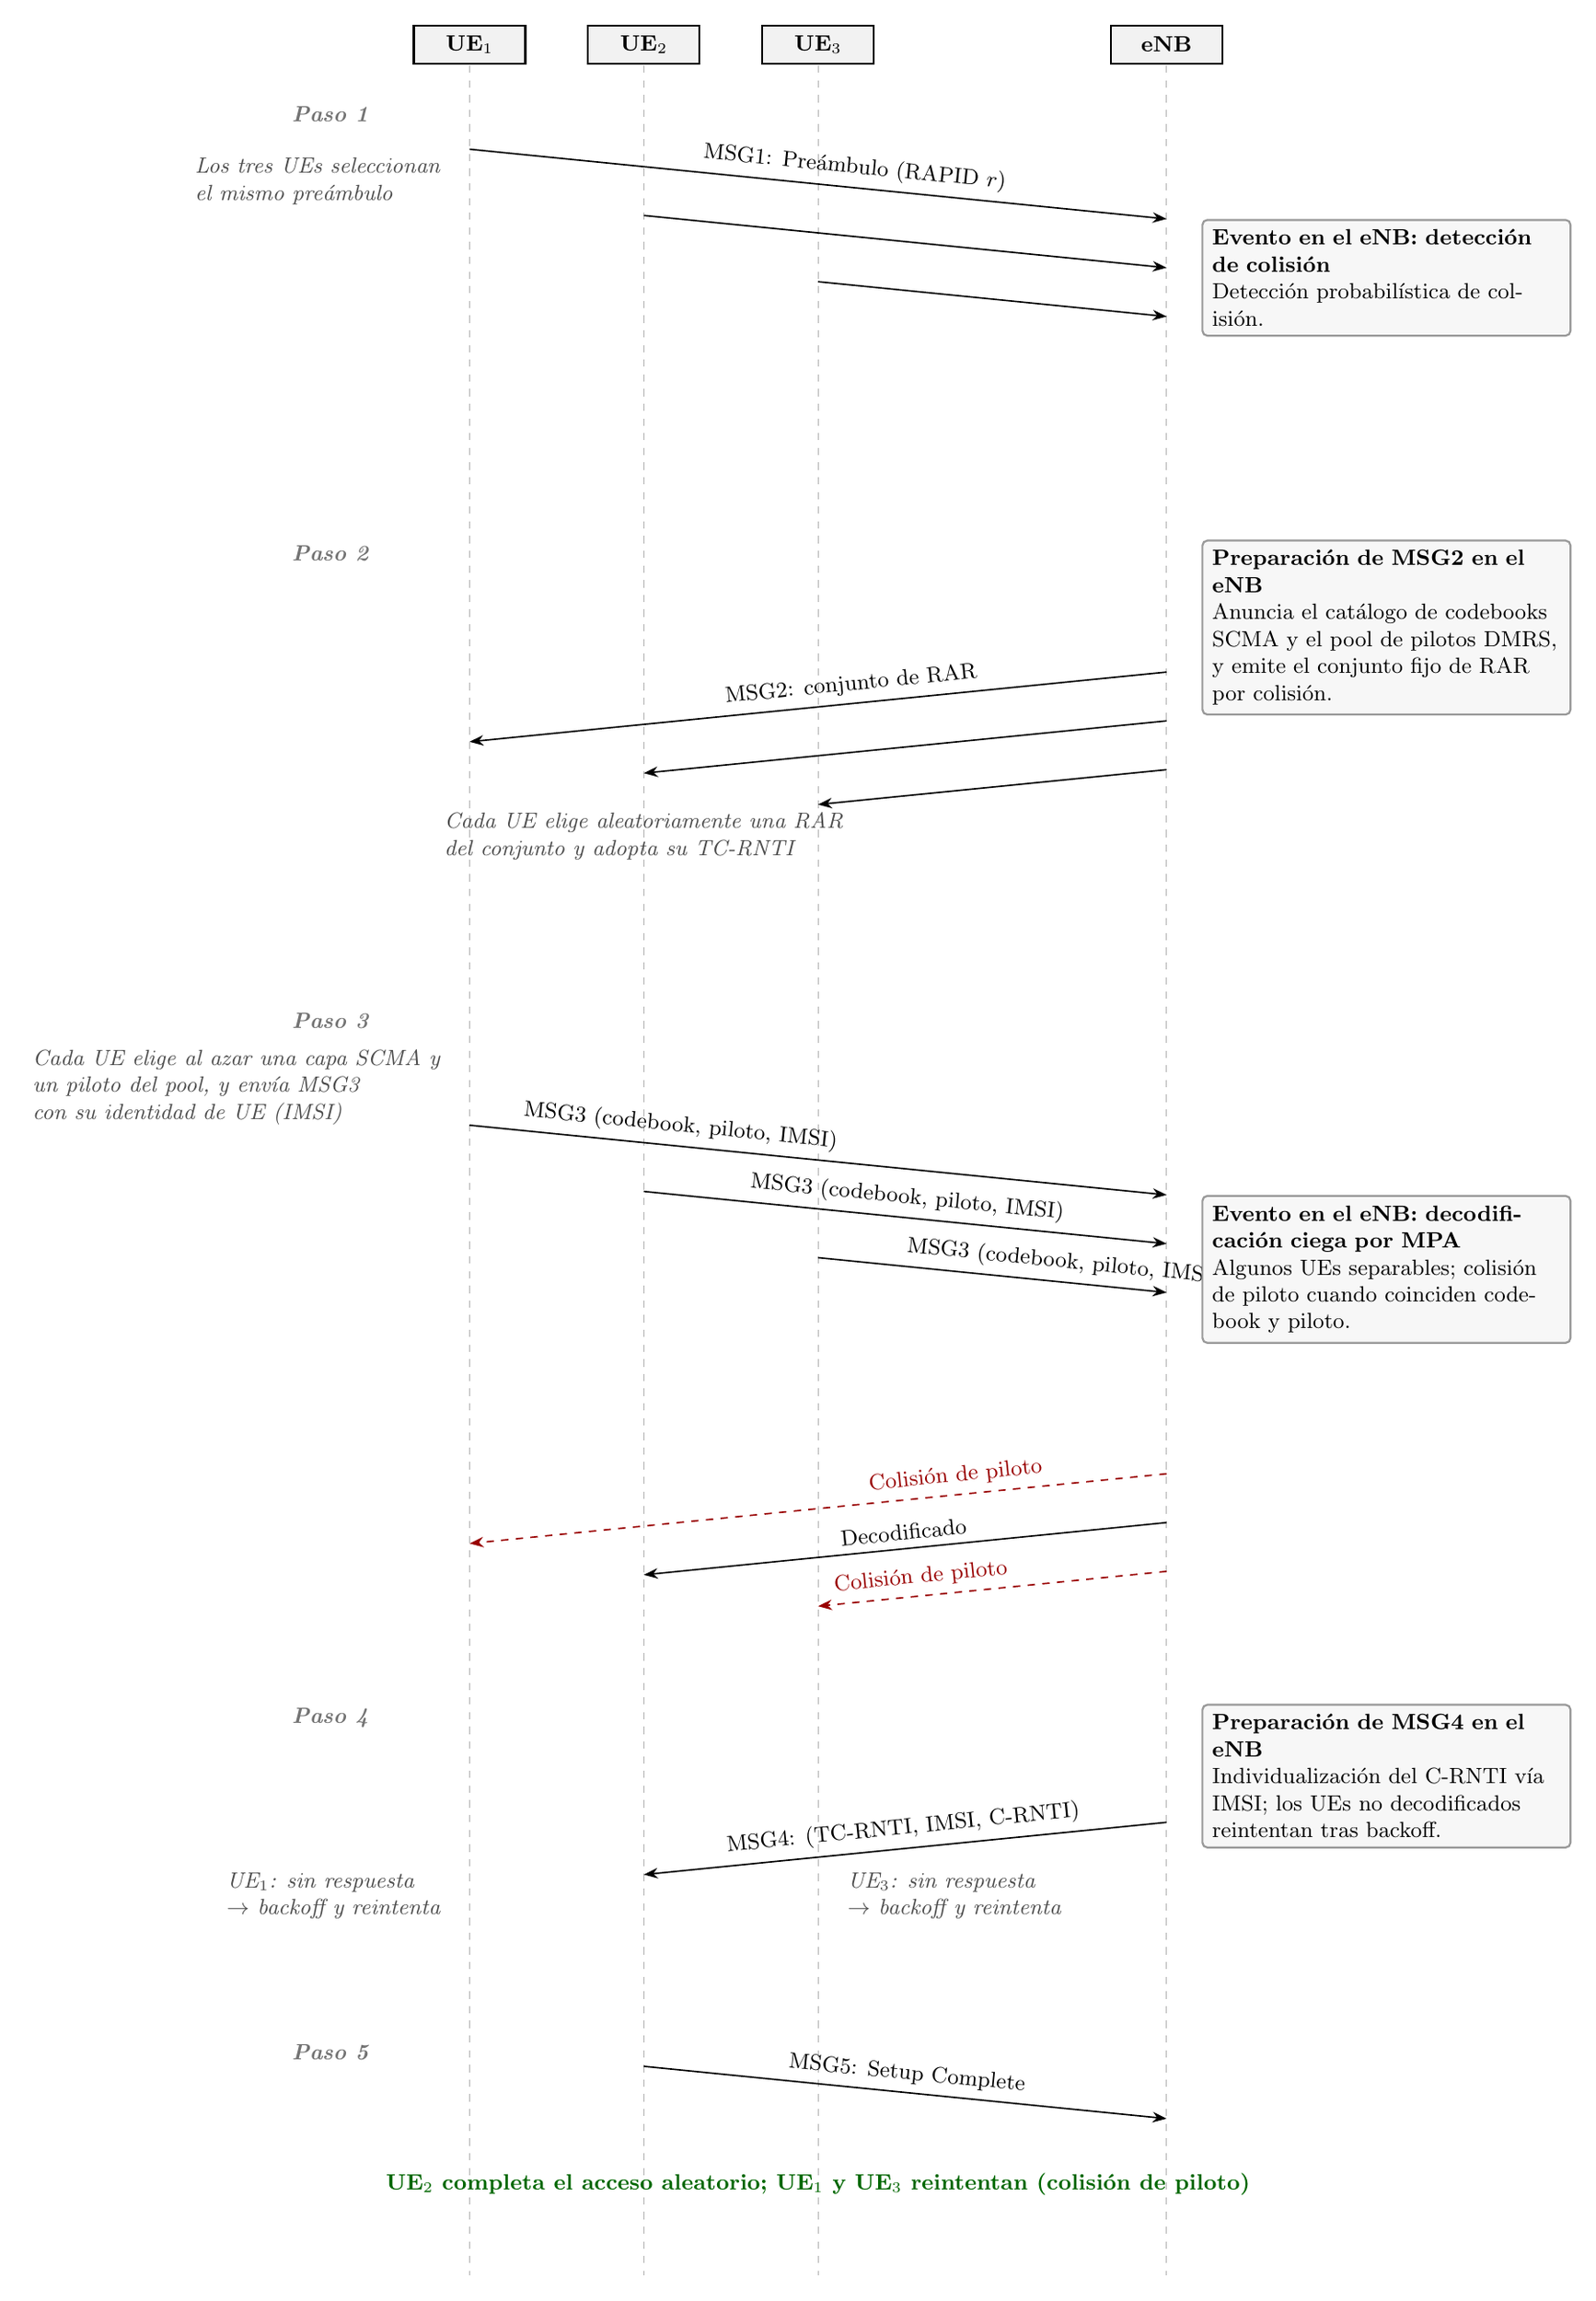
\begin{tikzpicture}[
    >=Stealth,
    font=\small,
    entity/.style={draw, rectangle, minimum width=1.6cm, minimum height=0.55cm,
                   fill=black!5, font=\small\bfseries, thick},
    msg/.style={->, semithick},
    sidenote/.style={font=\small\itshape, text=black!70, align=left},
    callout/.style={draw=black!40, fill=black!3, rounded corners=2pt,
                    inner sep=4pt, font=\small, align=left, thick=0.4pt,
                    text width=5cm},
    phase/.style={font=\small\bfseries\itshape, text=black!55},
]

% --- Entities ---
\node[entity] (ue1) at (0, 0) {UE$_1$};
\node[entity] (ue2) at (2.5, 0) {UE$_2$};
\node[entity] (ue3) at (5, 0) {UE$_3$};
\node[entity] (enb) at (10, 0) {eNB};

% --- Lifelines ---
\draw[dashed, black!30, thin] (0, -0.3) -- (0, -32);
\draw[dashed, black!30, thin] (2.5, -0.3) -- (2.5, -32);
\draw[dashed, black!30, thin] (5, -0.3) -- (5, -32);
\draw[dashed, black!30, thin] (10, -0.3) -- (10, -32);

% ============================================================
% STEP 1: MSG1 (UE → eNB, slope -0.1, y-intercept spacing 0.7)
% UE1: (0,-1.5) → (10,-2.5)
% UE2: (2.5,-2.45) → (10,-3.2)   [y-int=-2.2]
% UE3: (5,-3.4)  → (10,-3.9)     [y-int=-2.9]
% ============================================================
\node[phase] at (-2.0, -1.0) {Paso 1};

\draw[msg] (0, -1.5) -- node[sloped, above, font=\small, pos=0.55]
    {MSG1: Preámbulo (RAPID $r$)} (10, -2.5);
\draw[msg] (2.5, -2.45) -- (10, -3.2);
\draw[msg] (5, -3.4) -- (10, -3.9);

\node[sidenote, anchor=north east] at (-0.3, -1.5)
    {Los tres UEs seleccionan\\el mismo preámbulo};

\node[callout, anchor=north west] at (10.5, -2.5) {
    \textbf{Evento en el eNB: detección de colisión}\\
    Detección probabilística de colisión.
};

% ============================================================
% STEP 2: MSG2 (eNB → UE, slope +0.1, y-intercept spacing 0.7)
% UE1: (10,-9.0) → (0,-10.0)
% UE2: (10,-9.7) → (2.5,-10.45)
% UE3: (10,-10.4) → (5,-10.9)
% ============================================================
\node[phase] at (-2.0, -7.3) {Paso 2};

\node[callout, anchor=north west] at (10.5, -7.1) {
    \textbf{Preparación de MSG2 en el eNB}\\
    Anuncia el catálogo de codebooks SCMA
    y el pool de pilotos DMRS, y emite el
    conjunto fijo de RAR por colisión.
};

\draw[msg] (10, -9.0) -- node[sloped, above, font=\small, pos=0.45]
    {MSG2: conjunto de RAR} (0, -10.0);
\draw[msg] (10, -9.7) -- (2.5, -10.45);
\draw[msg] (10, -10.4) -- (5, -10.9);

\node[sidenote, anchor=north] at (2.5, -10.9)
    {Cada UE elige aleatoriamente una RAR\\
     del conjunto y adopta su TC-RNTI};

% ============================================================
% STEP 3: MSG3 (UE → eNB, slope -0.1, y-intercept spacing 0.7)
% UE1: (0,-15.5) → (10,-16.5)
% UE2: (2.5,-16.45) → (10,-17.2)
% UE3: (5,-17.4) → (10,-17.9)
% ============================================================
\node[phase] at (-2.0, -14.0) {Paso 3};

\node[sidenote, anchor=north east] at (-0.3, -14.3)
    {Cada UE elige al azar una capa SCMA y\\
     un piloto del pool, y envía MSG3\\
     con su identidad de UE (IMSI)};

\draw[msg] (0, -15.5) -- node[sloped, above, font=\small, pos=0.3]
    {MSG3 (codebook, piloto, IMSI)} (10, -16.5);
\draw[msg] (2.5, -16.45) -- node[sloped, above, font=\small, pos=0.5]
    {MSG3 (codebook, piloto, IMSI)} (10, -17.2);
\draw[msg] (5, -17.4) -- node[sloped, above, font=\small, pos=0.7]
    {MSG3 (codebook, piloto, IMSI)} (10, -17.9);

\node[callout, anchor=north west] at (10.5, -16.5) {
    \textbf{Evento en el eNB: decodificación ciega por MPA}\\
    Algunos UEs separables; colisión de
    piloto cuando coinciden codebook y
    piloto.
};

% ============================================================
% Outcomes (eNB → UE, slope +0.1, y-intercept spacing 0.7)
% UE1: (10,-20.5) → (0,-21.5)
% UE2: (10,-21.2) → (2.5,-21.95)
% UE3: (10,-21.9) → (5,-22.4)
% ============================================================
\draw[->, semithick, red!60!black, dashed] (10, -20.5) --
    node[sloped, above, font=\small, text=red!60!black, pos=0.3]
    {Colisión de piloto} (0, -21.5);
\draw[msg] (10, -21.2) -- node[sloped, above, font=\small, pos=0.5]
    {Decodificado} (2.5, -21.95);
\draw[->, semithick, red!60!black, dashed] (10, -21.9) --
    node[sloped, above, font=\small, text=red!60!black, pos=0.7]
    {Colisión de piloto} (5, -22.4);

% ============================================================
% STEP 4: MSG4 (single arrow to UE2)
% ============================================================
\node[phase] at (-2.0, -24.0) {Paso 4};

\node[callout, anchor=north west] at (10.5, -23.8) {
    \textbf{Preparación de MSG4 en el eNB}\\
    Individualización del C-RNTI vía IMSI;
    los UEs no decodificados reintentan
    tras backoff.
};

\draw[msg] (10, -25.5) -- node[sloped, above, font=\small]
    {MSG4: (TC-RNTI, IMSI, C-RNTI)} (2.5, -26.25);

\node[sidenote, anchor=north east] at (-0.3, -26.1)
    {UE$_1$: sin respuesta\\
     $\rightarrow$ backoff y reintenta};

\node[sidenote, anchor=north west] at (5.3, -26.1)
    {UE$_3$: sin respuesta\\
     $\rightarrow$ backoff y reintenta};

% ============================================================
% STEP 5: MSG5
% ============================================================
\node[phase] at (-2.0, -28.8) {Paso 5};

\draw[msg] (2.5, -29.0) -- node[sloped, above, font=\small]
    {MSG5: Setup Complete} (10, -29.75);

\node[font=\small\bfseries, text=green!40!black] at (5, -30.7)
    {UE$_2$ completa el acceso aleatorio; UE$_1$ y UE$_3$ reintentan (colisión de piloto)};

\end{tikzpicture}
\end{document}
